\documentclass[journal, letterpaper]{IEEEtran}

\usepackage{graphicx}
\usepackage[english]{babel}
\usepackage[square,numbers,super]{natbib}
\bibliographystyle{abbrvnat}

\usepackage{ mathrsfs }
\usepackage{braket}
\usepackage{url}        
\usepackage{amsmath}   
\usepackage{amssymb}
\usepackage{textgreek}	% Greek to me, dawg
\usepackage{listings}
\usepackage{csvsimple}
\usepackage{longtable}
\usepackage{siunitx}
\begin{document}
    
	\title{% 
                Quantum Information Processing 101 Project
                %\large Literature review of the 
            }

	\author{Roberto Scardia, Gabriele Lecce, Mirko Genoni}
	\maketitle

\section{Introduction}
In this literature review, we will lay out the necessary quantum mechanics and quantum information concepts needed to understand the meaning and consequences of Holevo's bound for quantum information theory. We will also show that classical information theory is a particular case of quantum information theory.
    
\section{Quantum mechanics}

Reasonably, a treatise on quantum mechanics should start with the definition of quantum states: historically, they evolved from the classical concept of "state" for a dynamic system. In classical physics, to describe the evolution of a dynamic system, it is not sufficient to know only the physical law that governs that particular system. It is also required to use the information given by the values of the state variables that describe the system and, in general, it is possible to organize these values inside a "state vector". 
In the same way, a "quantum state" is the mathematical entity that embeds the information needed to describe the evolution of a quantum system.\\ 
Quantum mechanics is the mathematical theory that describes the preparation, evolution, and measurement of a quantum system. By itself, quantum mechanics does not describe the physical law that a particular quantum system must obey, but it is useful as a framework to develop the mathematical foundation of other physical theories. Indeed, we will not reference any specific physical implementation while talking about quantum states, qubits, and measurements but we will stop at the general mathematical description.
The most useful mathematical representation of a quantum state for quantum information is the vector representation: in the same way classical states can be organized in vectors, the quantum states are thought to be components of a Hilbert space equipped with a scalar product. 
A Hilbert space is the generalization of the classical Euclidean vector space to possibly infinite dimension spaces where the classical ideas of (but not limited to) scalar product, distance, Pythagorean theorem, and Cauchy-Schwarz inequality still hold. The need for infinite dimension Hilbert space in quantum mechanics presents itself in case, for example, of the more known wave representation of quantum states, however, it is not strictly needed in our review for it will be shown that quantum information theory limits its scope to systems described by two-dimensional Hilbert space. 
In the vector representation, an isolated quantum state is a uni-dimensional sub-space of a Hilbert space $\mathscr{H}$: every vector $\ket{\psi} \in \mathscr{H}$ represents a different state apart from a complex constant $\lambda$, and every vector belonging to the same "line" or "ray" represents the same (isolated) quantum state. 
This kind of isolated state (i.e. not considered in an ensemble with other quantum states) is called a pure state and, in general, it is regarded as its representative vector an element of its sub-space with norm one, i.e $\bra{\psi}\ket{\psi} = 1$. Note that multiple such normalized vectors exist and are distinguished by a pure phase factor $e^i\phi$. Hence we can affirm that a pure quantum state, in reality, is a member of a projective Hilbert space, defined from a Hilbert space $H$ as the set of the equivalence classes $[v]$ of $ v \neq 0 \in \mathscr{H}$ with the equivalence relationship $\sim$ such that \( \forall v, w \in \mathscr{H} \: v \sim w \iff \exists\lambda \in \mathbb{C}\:|\: w = \lambda v \).
What we described in the previous section is the first postulate of quantum mechanics: \\ \\
\begin{minipage}{\linewidth}
    \textbf{Postulate 1}: Associated to any isolated physical system is a complex vector space with inner product (that is, a Hilbert space) known as the state space of the system. The system is completely described by its state vector, which is a unit vector in the system’s state space. \cite{chuang}
\end{minipage}\\ \\

From the theory of linear algebra, it is known that every element belonging to a vector (Hilbert) space can be expressed as a linear combination of the basis of the same space.
\[\mathscr{H} = \mathscr{L} \{B_{\mathscr{H}}\}\]
In quantum mechanics, this property of Hilbert spaces is called "superposition": each state can be expressed as the superposition of different states multiplied by a complex constant.\\
We said earlier that quantum information limits its scope to two-dimensional state space: the elements of such spaces are called qubits (from the portmanteau of quantum bits). Typically the canonical basis of a qubits space is denoted as \[\ket{0} = \begin{bmatrix}
           1 \\
           0 \\
           \end{bmatrix},
\ket{1} =  \begin{bmatrix}
           0 \\
           1 \\
           \end{bmatrix}\] 
but others are known such as the computational basis \[\ket{+} = (\ket{0} - \ket{1})\frac{1}{\sqrt{2}} \]
\[\ket{-} = (\ket{0} + \ket{1})\frac{1}{\sqrt{2}} \]

In general, a pure quantum state is nearly impossible to be physically realized and we have to resort to a probabilistic description of our quantum system. These uncertain states are called "mixed states" and arise not only in the preparation of real quantum systems but also in the case of entangled states.\\ 
Such description can be obtained by modeling it as an ensemble of pure quantum states $\psi_{i}$ with a priori probabilities $p_i$ using the concept of density operator $\rho$: 
 \[\rho = \sum_{i}p_i\ket{\psi_i}\bra{\psi_{i}}\]
The density operator can also be defined for a pure state $\psi$ as: 
\[\rho_\psi = \ket{\psi}\bra{\psi}\]
 
That can be generalized in the case that our quantum system is in a mixed state:
\[\rho = \sum_i p_i \rho_i\]
Where $\rho_i$ is the density operator of the pure states that compose the ensemble. It's easy to verify that $\rho$ is always positive and its trace is equal to one. 

Mixed states are not to be confused with the superposition of states: superposition results from the linearity of the operator that governs the quantum processes and no probability is involved until the measurement of such states occurs.

We said earlier that quantum mechanics does not describe the physical laws that govern the physical systems taken into consideration, but gives an important description in the form of its second postulate:\\

\begin{minipage}{0.96\linewidth}
\textbf{Postulate 2}: The evolution of a closed quantum system is described by a unitary
    transformation. That is, the state $\ket{\psi}$ of the system at time $t_1$ is related to the state $\ket{\psi}'$
    of the system at time $t_2$ by a unitary operator U which depends only on the times $t_1$ and $t_2$ \cite{chuang}
\end{minipage} \\ \\

Note that the postulate does not state anything about U other than it being a unitary operator. A unitary operator $U$ is a linear operator defined on a Hilbert space such that $UU^\dagger = U^\dagger U = I$. Note that U is a linear operator and this comes in handy when considering the superposition principle: having decided a basis, each operator can be defined as the matrix of the column images of the basis elements.\\
We will not dwell on every mathematical implication of this definition but it will be useful later to cite the alternative postulation involving the \textit{Schr{\"o}dinger's equation}:\\ \\

\begin{minipage}{0.96\linewidth}
\textbf{Postulate 2'}: The time evolution of the state of a closed quantum system is described by the \textit{Schr{\"o}dinger's equation}, \[i\hbar\frac{d\ket{\psi}}{dt} = H\ket{\psi}\] In this equation, $\hbar$ is a physical constant known as Planck’s constant whose value must be experimentally determined. The exact value is not important to us. In practice, it is common to absorb the factor $\hbar$ into $H$, effectively setting $\hbar$ = 1. $H$ is a fixed Hermitian operator known as the Hamiltonian of the closed system. \cite{chuang}
\end{minipage} \\ \\
The Hamiltonian is the operator related to the total energy of the quantum system taken into consideration and its expression is dependent on the physical description of the system; i.e. quantum mechanics still does not describe the physical law of the system but just their properties.

What our discussion on quantum mechanics lacks at this point is a description of what happens during the measurement process: when a quantum state is measured, the quantum system has to interact with the measurement apparatus so it cannot be considered a closed quantum system and the second postulate cannot be considered valid. In the same way that QM doesn't describe the laws involved with the evolution of the system, it does not prescribe a particular apparatus or practical procedure to carry out a quantum measure but lays out the mathematical foundation to describe the results.\\
The third and last postulate of QM states the following:\\ \\

\begin{minipage}{0.96\linewidth}
\textbf{Postulate 3}:  Quantum measurements are described by a collection {$M_m$} of measurement operators. These are operators acting on the state space of the system being measured. The index $m$ refers to the measurement outcomes that may occur in the experiment. If the state of the quantum system is $\ket{\psi}$ immediately before the measurement then the probability that result $m$ occurs is given by
\[p(m) = \bra{\psi}M^\dagger_m M_m\ket{\psi}\]
and the state of the system after the measurement is
\[\frac{M_m\ket{\psi}}{\bra{\psi}M^\dagger_m M_m \ket{\psi}}\]
The measurement operators satisfy the completeness equation,
\[\sum_m M^\dagger_m M_m = I\]
The completeness equation expresses the fact that probabilities sum to one:
\[ \sum_m p(m) = \sum_m \bra{\psi}M^\dagger_m M_m\ket{\psi}=1\cite{chuang}\]
\end{minipage} \\ \\
The states here are considered to have norm equal to one.
A quantum measure involves necessarily a probabilistic description: while in classical physics we need a statistical description (being classical or Bayesian) to account for noise and measurement error, in QM the result of the measurement operation is intrinsically probabilistic. 
For example, a valid example of measurement operator collection on qubits is the set composed by the density operator of the canonical basis, \(M_0 = \ket{0}\bra{0}\), \(M_1 = \ket{1}\bra{1}\). If we consider a state $\psi = a\ket{0} + b\ket{1}$ the probability of measuring the state 0 or 1 is:
\[p(0/1) = \bra{\psi}M_{0/1}^\dagger M_{0/1} \ket{\psi} = \bra{\psi} M_{0/1} \ket{\psi} = |a/b|^2\] 
where the hermiticity property of the density operator $(M_{0/1} =M_{0/1}^\dagger, M_{0/1}^2=M_{0/1}$ is used. 
In this specific example, we choose to use the density operator of two orthogonal states ($\bra{0}\ket{1} = 0$, by definition of canonical basis) and if the state $\psi$ were equal to 0 or 1 we would have been able to measure 0 or 1 with probability 1 respectively. However, this is only true for states that are orthogonal, and, in general, for two states that are not orthogonal it does not exist a measurement set with this property. For this reason, two states that are not orthogonal are called \textit{non-distinguishable states}.\\
In general, the operators in the measurement set do not have to be unitary. In case they possess this property (i.e. the second postulate is respected during the measurement) and are orthogonal ($M_mM_n = 0 \; for\; m \neq n$) we are in the special case of \textit{projective measurement}. In projective measurement, an operator $M$ called \textit{observable} is defined with spectral decomposition \[M = \sum_m mP_m\] where $m$ is one of its eigenvalue and $P_m$ the orthogonal projectors over its eigenspaces; those compose the measurement set. The previous example can be understood as a case of projective measurement and the same simplifications for calculating the probability distribution can be applied:
\[ p(m) = \bra{\psi}P_m\ket{\psi}\] The resulting state after a projective measurement is \( \frac{P_m\ket{\psi}}{\sqrt{p(m)}}\) i.e. one of the states described by the eigenspaces of $M$.\\   
Another special case of the third postulate that is thoroughly used in quantum information is the Positive Operator-Value Measure: instead of singularly choosing the measurement operators $M_m$ such that they respect the completeness equation as a measurement set whatever choice of $E_m$ such that \(\sum_m E_m = I\). This formalism is useful whenever after the measure there is no interest in the state of the system or the measurement is not repeatable. By definition, projective measurement describes a repeatable procedure: after obtaining the state $\ket{\phi_m}$ as the result of the measure by repeating the measurement with the same set we re-obtain $\ket{\phi_m}$ with probability one. In quantum information we are often only interested in the statistics of the measure and not in the evolution of the system and the utility of this formalism will be shown in the following paragraphs.
\\ 
\\
A quantum phenomenon that plays an important role in both quantum information theory and quantum cryptography is the no-cloning theorem. Suppose that we have a device that can duplicate quantum states: 
if we want to copy a pure state $\ket{\psi}$ in a blank state $\ket{X}$ we have to apply a unitary operator on the system: 
\[U\ket{\psi}\ket{X} = \ket{\psi}\ket{\psi} \]
And this is true for all the orthogonal $\ket{\psi_i}$ forming a space vector. However, it's not possible to duplicate a non-orthogonal state \cite{clone} e.g. $\ket{\psi} = \frac{1}{\sqrt{2}}(\ket{0}+\ket{1})$: 
\[U\frac{1}{\sqrt{2}}(\ket{0}+\ket{1})\ket{X} = U\frac{1}{\sqrt{2}}(\ket{0}\ket{X}) + U\frac{1}{\sqrt{2}}(\ket{1}\ket{X}) = \] \[=\frac{1}{\sqrt{2}}\ket{0}\ket{0} +\frac{1}{\sqrt{2}}\ket{1}\ket{1}\]
That is different from what we expected: 
\[ \frac{1}{\sqrt{2}}{(\ket{0}+\ket{1})\frac{1}{\sqrt{2}}}(\ket{0}+\ket{1}) \neq  \frac{1}{\sqrt{2}}\ket{0}\ket{0} +\frac{1}{\sqrt{2}}\ket{1}\ket{1}\]
\section{Quantum information}
In “classical” information theory Shannon’s entropy is defined as the measure of information of a memory-less stationary source, for which we know the probability $P(X)$ of a set of symbols \{X\}: \[H(X) = - \sum_{X} P(X)\log_2P(X)\]
To describe a set of quantum states \{$\psi$\}, probability distributions are replaced by density operators. The natural extension of the Shannon’s entropy is the Von Neumann entropy, defined as:
\[S(\rho) = -tr(\rho \log\rho) = -\sum_{\psi} \lambda_{\psi}\log\lambda_{\psi} \]
Where $\lambda_{\psi}$ are the eigenvalues of the density operator $\rho$. 
We can easily verify that if the states of the alphabet are orthogonal (e.g. $\{X\} = \{\ket{0},\ket{1}\}$), the Von Neumann entropy coincides with Shannon's entropy: 
\[\rho = p\ket{0}\bra{0} + (1-p)\ket{1}\bra{1} = \begin{bmatrix}
    p & 0 \\
    0 & 1-p
\end{bmatrix}\]
\[\Rightarrow S(\rho) = -p\log_2p -(1-p)\log_2(1-p) = \log_2\frac{(1-p)^{p-1}}{p^p} \]
That coincides with Shannon's entropy of a binary source. Suppose the dimension d of the space vector $C^d$ can be considered as the number of symbols in a classical alphabet. In that case, the Von Neumann entropy is upper bounded by: \[S(\rho) \le log_2(d) \] And in general, for an ensemble of non-orthogonal pure quantum states (in this case $\rho$ is not hermitian) we have: \[S(\rho) \le H(X)\] It is possible to verify that the single pure state $i$ of the ensemble has the property $S(\rho_i) = 0$. In the most general case, when an ensemble of mixed states describes our system, we have the following upper bound: 
\[S(\rho) \le \sum_{i}p_iS(\rho_i) + H(X)\] that is held with equality only when the states $\rho_i$ have orthogonal support. If we rewrite the last expressions as follows: 
\[S(\rho) - \sum_{i}p_iS(\rho_i) \le  H(X)\]
We can identify a quantity: \[\chi(\rho_i) = S(\rho) - \sum_{i}p_iS(\rho_i)\] that is the Holevo information of our ensemble. This quantity can be regarded as a generalization of the Von Neumann entropy when we send messages constructed from an alphabet of non-orthogonal mixed states. It will play an important role when we will describe the Holevo's bound.
\\
\\
When we use non-orthogonal states, a new “quantum” problem arises. Suppose that our source can only send symbols from an ensemble of two non-orthogonal states e.g. \{$\ket{0}, \frac{\ket{0}+\ket{1}}{\sqrt{2}}$\} and we want to measure them with a set {E} of POVM elements. We can define: \[E_1 = \frac{\sqrt{2}}{1+\sqrt{2}}\ket{1}\bra{1},\] \[E_2 = \frac{\sqrt{2}}{1+\sqrt{2}}\frac{(\ket{0}-\ket{1})(\bra{0}-\bra{1})}{2}\] such that we always have state $\frac{\ket{0}+\ket{1}}{\sqrt{2}}$ when we measure $E_1$ and state $\ket{0}$ when we measure $E_2$. However the set \{$E_1,E_2$\} does not satisfy completeness relation $\sum_mE_m = I$, which is only satisfied by adding a third operator $E_3 = I- E_1-E_2$, that gives no information about the identity of the measured the state: \[\bra{\psi_i}E_3\ket{\psi_i} \neq 0,1 \] That means that if we use non-orthogonal states we don't have perfect reliability. This is the accessible information problem, and can be seen as a direct consequence of the no-cloning theorem. This is never seen in classical information theory, since its symbols are always pure orthogonal states. To quantify how can we know about the accessible information, we can use another classical information theory concept known as mutual information: 
\[I(X,Y) = H(X) - H(X|Y)\]
This is a measurement of the degree of correlation between two random variables, in our case the state measured is Y and the state sent is X. In classical noiseless channels, the mutual information is always equal to the Shannon entropy of the source, since there isn't a problem with accessible information. We expect that in quantum information this inequality holds: \[I(X,Y) \le H(X)\]and it's satisfied with equality only when my quantum system is described by orthogonal pure states. In the next chapter, we wish to connect the Holevo quantity and the mutual information to get more general results. 



\section{Holevo's bound}

The Holevo's bound is one of the most important results in quantum information theory.
Suppose that one actor has prepared a quantum state with density operator $\rho_X$ choosing over $n$ different possible states with probability $p_x \; \; x \in [0,n]$. A second actor has then measured this state with a POVM set $E_y = {E_0, ..., E_y}$ with measure outcome Y. The Holevo's bound states that for such measurement:
\[I(X,Y) \leq S(\rho) - \sum_x p_xS(\rho_x) = \chi\]

where \(\rho = \sum_x p_x \rho_x \) and $\chi$ is the Holevo $\chi$ quantity. 

Using Holevo bound and the results from the previous chapter, we can relate the mutual information of a quantum source described by an alphabet of mixed states with Shannon's entropy of that source: 
\[ I(X,Y) \le \chi(\rho_i)\le H(X)\]
This means that the mutual information is strictly less than $H(X)$ when $\rho_i$ doesn't have orthogonal support, or in other words, when the mixed states of the alphabet are not orthogonal. This is the generalization of what was shown in the previous chapter for the simplified case of a quantum system with an alphabet of non-orthogonal pure states. 
\\
\\
To show the importance of the orthogonality of the mixed states, let's switch for a moment to a 3-dimensional Hilbert space. Suppose we take $\rho_i$ from the ensemble of pure orthogonal states ${X}=\{\ket{0},\ket{1},\ket{2}\}$.  We choose $\rho_1 = q\ket{0}\bra{0} + (1-q)\ket{1}\bra{1}$ and $\rho_2 = p\ket{1}\bra{1}+(1-p)\ket{2}\bra{2}$ to be the mixed states of our system. The density operator of the system is $\rho = \frac{1}{2}\rho_1 + \frac{1}{2}\rho_2$, so the Holevo quantity is upper bounded by the binary entropy: H(X) = 1. When $q=1$ or $p=0$, the mixed states are orthogonal, so we expect the Holevo quantity to be independent of respectively $p$ or $q$. We compute the Von Neumann entropies for this system: 

\[\rho_1 = \begin{bmatrix}
    q & 0 & 0 \\
    0 & 1-q & 0 \\
0 & 0 & 0
\end{bmatrix} \Rightarrow S(\rho_1) = H_2(q);\]
\\
\[\rho_2 = \begin{bmatrix}
    0 & 0 & 0 \\
    0 & p & 0 \\
0 & 0 & 1-p
\end{bmatrix} \Rightarrow S(\rho_2)=H_2(p);\]
\\
\[\rho = \begin{bmatrix}
    q & 0 & 0 \\
    0 & (1-q)+p & 0 \\
0 & 0 & 1-p
\end{bmatrix}\] 
\\
\[ \Rightarrow S(\rho)=-\frac{1}{2}[q\log(\frac{q}{2})+(1-p)\log(\frac{1-p}{2}) +(1-q+p)\log(\frac{1-q+p}{2})]\]
\[= 1+\frac{1}{2}(H_2(p)+H_2(q)+\log\frac{p^p(1-q)^{1-q}}{(1-q+p)^{1-q+p}}) \]
We can finally write the Holevo quantity $\chi$: 
\\
\[\chi(q,p) = S(\rho)-\sum_ip_i\rho_i = 1+\frac{1}{2}\log\frac{p^p(1-q)^{1-q}}{(1-q+p)^{1-q+p}} \]
\[\Rightarrow \chi(q,p) = 1+ G(q,p) \le H(X) = 1\]
And as we expected: \[G(1,p) = G(q,0) = \log_21 = 0 \Rightarrow \chi = 1 = H(X)\]
\begin{figure}[!h]
    \centering
    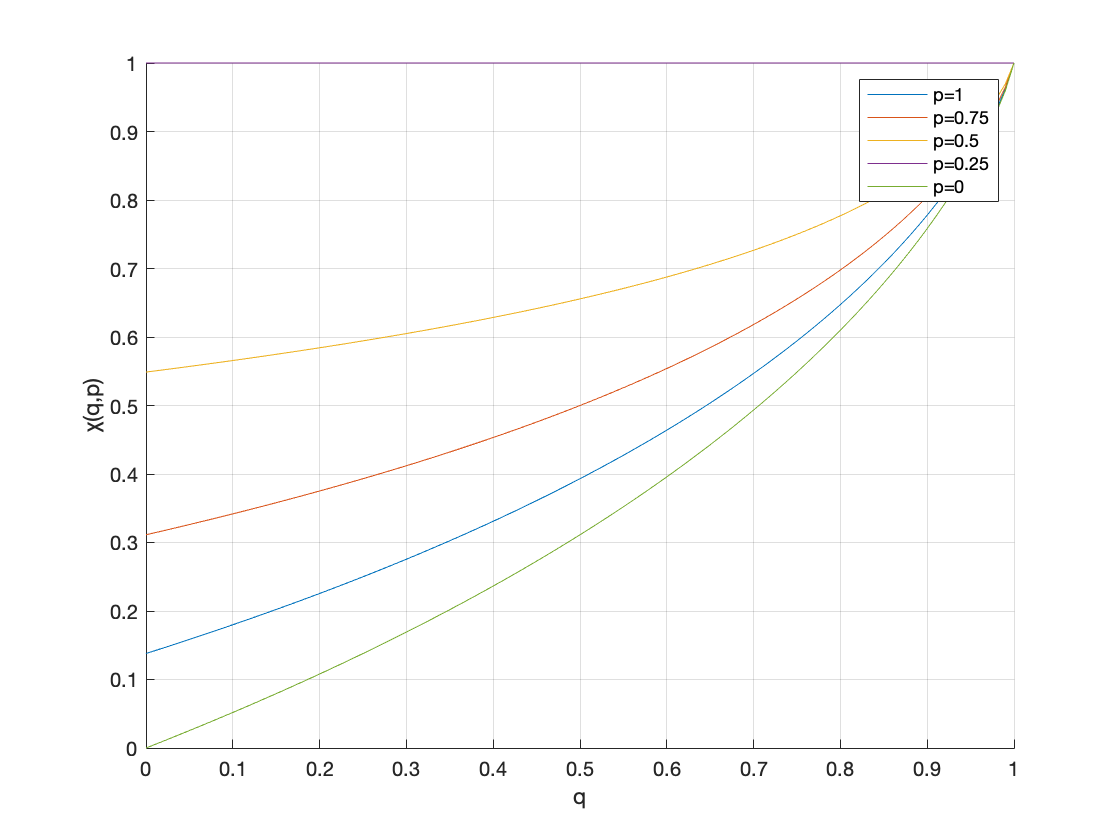
\includegraphics[width=0.5\textwidth]{graficus.png}
        \caption{Holevo quantity $\chi$ as function of q and p.}
     \label{fig:quadtree}
\end{figure} 
\\
If $p$ it's set and we increase $q$, the Holevo quantity increases because the mixed states approach the orthogonality condition. The mutual information of this quantum system is upper bounded by:
\[I(X,Y) \le 1\]
If we choose a proper POVM set and two orthogonal mixed states, we can achieve $I(X,Y) = 1$. Suppose to pick the particular case $\{X\} = \{\frac{1}{2}(\ket{0}+\ket{1}),\ket{2}\}=\{\ket{\psi_1},\ket{\psi_2}\}$, we can calculate the POVM as: 
\[\bra{\psi_1}E_1\ket{\psi_1} = 1 \Rightarrow E_1 = \begin{bmatrix}
    1 & 0 & 0 \\
    0 & 1 & 0 \\
0 & 0 & 0
\end{bmatrix} ;\]

  \[\bra{\psi_2}E_2\ket{\psi_2} = 1 \Rightarrow E_2 = \begin{bmatrix}
    0 & 0 & 0 \\
    0 & 0 & 0 \\
0 & 0 & 1
\end{bmatrix} \]
Where the completeness relation has been used to maximize the mutual information: 
\[ \sum_mE_m = E_1 + E_2 = I\]
We have found that optimal measurement determined by the ensemble has the property: 
\[p(m) = \delta_{m,x}\]
Where $\delta_{m,x}$ is the Kronecker delta. We can now better define the concept of accessible information as the maximization of the mutual information over all the sets $\{E_m\}$ of possible POVM measurements: 
\[I_{acc} = \max_{\{E_m\}}{I(X,Y)} \]

We have seen that orthogonal states are perfectly distinguishable, however it's not possible to maximize the mutual information in this way when the mixed states are non-orthogonal ($\chi <H(X)$). If we use an alphabet of pure states (to simplify the expression of $\chi$), we expect that: 
\[I(X,Y) \le \chi = S(\rho) < H(X)\]
Furthermore, it's also more complicated to guess what is the optimal POVM measurement.
In some cases we can exploit symmetries, for example, if we take an ensemble of pure states which have a three-fold symmetry e.g.: \\\[\{\psi_i\} =\{\cos(\frac{2\pi}{3}*n)\ket{0}+ \sin(\frac{2\pi}{3}*n)\ket{1}\} = \]\[\{\ket{0},-\frac{1}{2}\ket{0}+\frac{\sqrt{3}}{2}\ket{1},-\frac{1}{2}\ket{0}+-\frac{\sqrt{3}}{2}\ket{1}\}\]
with n=0,1,2 and the same a priori probabilities, it is possible to construct an optimal POVM with the same symmetry, that achieves: \[I_{acc} \simeq 0.58496 < S(\rho) = 1\cite{caltech}\] We could try and group states in a similar way to classical information theory: \[\ket{\psi} = \ket{\psi_i}_1\ket{\psi_i}_2...\ket{\psi_i}_m\]
In this way, we would have $3^m$ possible "codewords". However, it is possible to demonstrate that the accessible information doesn't change. A better strategy is the Peres-Wootters method \cite{peres}: instead of using all the $3^m$ codewords built before, we just use three codewords formed by repeating m times one of the three pure states of the ensemble, e.g. for the first state: 
\[\ket{\psi_1} = \ket{0}_1\ket{0}_2...\ket{0}_m\]
In this way the three new states $\ket{\psi_i}$ are more distinguishable; for the case m = 2 we have an improvement of the Von Neumann entropy: 
\[S(\rho)_{m} = S(\rho)_{2} = 1.5 < H(X) = \log_23 \]
We can say that they are more distinguishable because the inner product with the other states is more orthogonal increasing $m$, in other words:  \[\bra{\psi_i}\ket{\psi_j}_m>\bra{\psi_i}\ket{\psi_j}_{m+1},  i \neq j\]
In fact for the $m=2$ case, we improve the maximum mutual information: 
\[I_{acc, m=2} = 1.36907 >  0.58496 \]
The most fundamental concept that the Peres-Wooters method highlights is that it's better to group qubits to create an alphabet with just the more distinguishable letters. Furthermore, we want to measure these states using a POVM constructed by a procedure called  PGM ("pretty good measurements")\cite{caltech}, which gives the maximization of the mutual information.
\\
\\We can also extend this method to an ensemble of non-orthogonal mixed states, saying that when $m\rightarrow \infty$ the accessible information tends to the Holevo's quantity: 
\[I_{acc,m\rightarrow\infty } \rightarrow \chi(\rho_i) \]
We can say, from what we have shown in this review, that the accessible information plays a role similar to the capacity of a channel in classical information theory: it tells us how many "classical" bits of information can be reliably transmitted over the channel. In order to have a good accessible information, we can maximize the Holevo's quantity by using longer codewords and by choosing the optimal POVM set of the system.


\begin{thebibliography}{3}

\bibitem{chuang}
M.A. Nielsen and I.L. Chuang, "Quantum Computation and Quantum Information", Cambridge University Press.
\bibitem{clone}
W.K. Wootters and W.H. Zurek, "A single quantum cannot be cloned", Nature, Volume 299, October 1982.
\bibitem{mixed}
Steven J. van Enk, "Mixed and pure states", notes of the course of quantum mechanics, University of Oregon, \url{https://pages.uoregon.edu/svanenk/solutions/Mixed_states.pdf}
\bibitem{caltech}
John Preskill, "Quantum Information Theory", notes of the course of quantum computation, California Institute of Technology, \url{http://theory.caltech.edu/~preskill/ph229/notes/chap5.pdf} 
\bibitem{john}
John Wright, "Lecture 18: Quantum Information Theory and Holevo’s Bound", notes of the course of Quantum Computation and Information, Carnegie Mellon University, \url{https://www.cs.cmu.edu/~odonnell/quantum15/lecture18.pdf}
\bibitem{peres}
Asher Peres and William K. Wootters, "Optimal Detection of Quantum Information", Physical Review Letters, vol. 66, num. 9, 04 March 1991.

\end{thebibliography}

\end{document}